\documentclass{article}

% if you need to pass options to natbib, use, e.g.:
%     \PassOptionsToPackage{numbers, compress}{natbib}
% before loading neurips_2024


% ready for submission
\PassOptionsToPackage{numbers}{natbib}
\usepackage[preprint]{neurips_2024}


% to compile a preprint version, e.g., for submission to arXiv, add add the
% [preprint] option:
%     \usepackage[preprint]{neurips_2024}


% to compile a camera-ready version, add the [final] option, e.g.:
%     \usepackage[final]{neurips_2024}


% to avoid loading the natbib package, add option nonatbib:
%    \usepackage[nonatbib]{neurips_2024}
\usepackage[table]{xcolor}
\usepackage{amsmath}
\usepackage{subcaption}
\usepackage{graphicx}
\usepackage{float}
\usepackage[utf8]{inputenc} % allow utf-8 input
\usepackage[T1]{fontenc}    % use 8-bit T1 fonts
\usepackage{hyperref}       % hyperlinks
\usepackage{url}            % simple URL typesetting
\usepackage{booktabs}       % professional-quality tables
\usepackage{amsfonts}       % blackboard math symbols
\usepackage{nicefrac}       % compact symbols for 1/2, etc.
\usepackage{microtype}      % microtypography
% xcolor already loaded with [table] option above
\usepackage{tikz}
\usetikzlibrary{arrows.meta}


\title{Non-Axiomatic Reasoning for Longitudinal Identity Resolution: NARS on ICE-ID and Standard ER Benchmarks}


\author{%
   Gonçalo Hora de Carvalho\thanks{Corresponding author: \texttt{goncalo@iiim.is}} \\
  IIIM, Iceland \\
  \texttt{goncalo@iiim.is} \\
  \And
  Lazar S.~Popov \\
  IIIM, Iceland \\
  \And
  Sander Kaatee \\
  IIIM, Iceland \\
  \AND
  Kristinn R.~Thórisson \\
  Full Research Professor, Department of Computer Science\\
  Reykjavik University\\
  \And
  Tangrui Li \\
  Temple University\\
  \And
  Pétur Húni Björnsson \\
  Department of Nordic Studies and Linguistics\\
  University of Copenhagen\\
  \And
  Jilles S.~Dibangoye \\
  Associate Professor, Machine Learning Group, Department of Artificial Intelligence\\
  Bernoulli Institute, University of Groningen\\
}


\begin{document}


\maketitle


\begin{abstract}
We evaluate OpenNARS-for-Applications (ONA) for longitudinal identity resolution on Icelandic historical census data spanning 220 years (1703--1920), while benchmarking it on standard entity resolution datasets (Abt--Buy, Amazon--Google, DBLP--ACM, DBLP--Scholar) \cite{Kopcke2010, mudgal2018deep}. NARS is a general-purpose AI framework designed to reason with limited knowledge and resources; its core is Non-Axiomatic Logic (NAL), a term-based logic. Our experiments show that this evidence-based symbolic matcher can serve as a transparent baseline alongside classical probabilistic linkage and modern neural matchers. We report pairwise metrics, calibration sensitivity, and a deployment-faithful candidate-graph evaluation on ICE-ID, and compare against strong baselines across standard ER datasets.
\end{abstract}

%%%%%%%%%%%%%%%%%%%%%%%%%% INTRODUCTION %%%%%%%%%%%%%%%%%%%%%%%%%% 

\section{Introduction}

Linking historical census records is an important step in research on social mobility, demographic change, migration, and epidemiology, yet it remains arduous because names mutate, fields are missing, and administrative borders shift over time \cite{ruggles2018historical, bailey2020}.  
While supervised matchers trained on labeled pairs improved accuracy for nineteenth-century U.S.\ censuses \cite{feigenbaum2016}, most census-specific benchmarks still oversimplify the problem: they cover only short time ranges (often a single decade), omit kinship structure, and treat geography as flat text rather than a hierarchy \cite{papadakis2023}.  

Benchmark design strongly shapes progress in entity resolution and record linkage. We release \textbf{ICE-ID} to fill a missing setting: long-horizon longitudinal person matching with temporal drift, hierarchical geography, and expert-curated identity clusters.  
Spanning 16 Icelandic census waves (1703--1920) and covering more than 220 years, ICE-ID contains 984\,028 rows and 226,864 expert-curated person clusters.  

We formulate two tasks:

\begin{enumerate}
  \item \textbf{Intra-census linkage}: identify the same individual within a single census.
  \item \textbf{Cross-census linkage}: identify the same individual across successive censuses despite spelling drift and age progression.
\end{enumerate}

Train/validation/test splits follow a strictly temporal protocol: rows up to 1870 for training, 1871--1890 for validation, and 1891--1920 for held-out testing, mirroring real archival workflows.  
Evaluation combines pairwise metrics (precision, recall, F$_1$, ROC-AUC) with clustering quality (Adjusted Rand Index, ARI).

We benchmark several model families:

\begin{itemize}
  \item \emph{Classical probabilistic linkage}: Fellegi--Sunter and deterministic rule-based matchers;
  \item \emph{Symbolic reasoning}: a Non-Axiomatic Reasoning System (NARS) that learns identity rules from streaming examples;
  \item \emph{Neural matchers}: Ditto \cite{Li2020DeepEM}, HierGAT \cite{yao2022hiergat}, and zero-shot/LLM-based methods (AnyMatch \cite{zhang2024anymatch}, MatchGPT).
\end{itemize}

Our results show that NARS achieves competitive pairwise accuracy (F$_1$=0.994 on ICE-ID) using only symbolic judgment-based scoring, without deep representation learning or GPU resources. On standard ER benchmarks (DBLP--ACM, DBLP--Scholar), NARS matches or exceeds reported state-of-the-art F$_1$, while remaining below SOTA on product-matching datasets (Abt--Buy, Amazon--Google).
These findings suggest that symbolic reasoning can serve as a strong, transparent baseline for entity resolution, and motivate \emph{hybrid} pipelines that fuse symbolic and neural evidence.

%%%%%%%%%%%%%%%%%%%%%%%%%% METHODS %%%%%%%%%%%%%%%%%%%%%%%%%%%%% 

\section{Methods}
\label{sec:methods}
This section describes the ICE-ID benchmark, the NARS matcher, baselines, and evaluation protocol.

\subsection{ICE-ID Benchmark}
We evaluate on ICE-ID \cite{iceid2024}, a benchmark of 984,028 Icelandic census records (1703--1920) with 226,864 expert-labeled person clusters. We use the canonical temporal splits (up to 1870 train / 1871--1890 validation / 1891--1920 test) and report pairwise metrics (Precision, Recall, F$_1$, AUC), clustering metrics (ARI, B$^3$), and ranking metrics (P@k, R@k). Full dataset documentation is in the companion data paper.

\subsubsection{Data Preparation}
Records are loaded from \texttt{people.csv} with string columns normalized to lowercase and numeric fields (\texttt{id}, \texttt{heimild}, \texttt{birthyear}, \texttt{person}, and geographic/kinship IDs) coerced to integers. Missing IDs are dropped; missing name fields are filled with empty strings. NARS and the symbolic matchers operate directly on these record pairs; the ML ensemble baseline uses pairwise TF-IDF features over concatenated record text. All ICE-ID experiments under the shared protocol use the same raw record representation and temporal splits keyed by \texttt{heimild}.

\subsubsection{Pair Construction and Sampling}
Positive pairs are drawn from expert-labeled clusters: two records share a positive label if they share the same \texttt{person} (or equivalent) ID. For \emph{cross-wave} linkage, the benchmark supports pair generation across distinct census-year windows (e.g., source and target year ranges) via the same cluster semantics. Negatives are formed by sampling pairs whose records belong to different clusters. We use a 2:1 negative-to-positive ratio when building the labeled set within each split. For ICE-ID, pair generation and any subsampling are performed \emph{inside} the fixed temporal splits (train: up to 1870, validation: 1871--1890, test: 1891--1920); no random train/validation/test split is applied across years. If the number of candidate pairs in a split exceeds 50,000, we uniformly subsample that split to the cap so that NARS and the ML baselines are evaluated on the same bounded pair set. The implementation uses a configurable cap of 50,000 pairs and does not impose a same-census-year constraint on negatives; within-wave evaluation can be obtained by restricting the record pool to a single \texttt{heimild} in a given run.

\subsection{ML Ensemble Baseline}

As a baseline, we compare against an ensemble of four tree-based classifiers (XGBoost, LightGBM, CatBoost, Random Forest) averaging match probabilities. The ensemble is trained on pairwise text-derived and structured comparison features computed from the same raw record pairs used by NARS. Model selection uses 10-fold cross-validation within the training split; final evaluation uses the same held-out validation and test splits as NARS. Full details are provided in the ICE-ID data paper.

\subsection{OpenNARS-for-Applications}

\textbf{Implementation:} We use OpenNARS-for-Applications (ONA) as the underlying NARS engine. ONA defines the judgment vocabulary and evidence framework; record pairs are converted into Narsese statements encoding attribute agreements and disagreements. The reported experiments use the LLR scoring instantiation described in the ``Practical scoring variant'' paragraph below.

\textbf{Algorithm Overview:} Figure~\ref{fig:algo} summarizes the procedure.

\begin{figure}[H]
  \centering
  \fbox{%
    \begin{minipage}{0.96\linewidth}
    \small\ttfamily
    \textbf{Inputs:} labeled training pairs (r1, r2, y), pool size P, patterns used n\\[0.5em]
    \textbf{1)} For each training pair:\\
    \hspace*{1em}J = preprocess(r1, r2) \hfill\textit{(atomic judgments)}\\
    \hspace*{1em}tv = TruthValue(f=y, c=0.9)\\
    \hspace*{1em}add/update (J $\rightarrow$ tv) in PatternPool (evict if $>$ P)\\[0.3em]
    \textbf{2)} Calibrate a threshold $\tau$ on held-out labeled pairs\\
    \hspace*{1em}(ICE-ID: median midpoint; classic ER: validation F$_1$)\\[0.3em]
    \textbf{3)} For each test pair:\\
    \hspace*{1em}Jq = preprocess(r1, r2)\\
    \hspace*{1em}select n reference patterns from pool (top/bottom expectation)\\
    \hspace*{1em}score = revise evidence from overlaps between Jq and selected patterns\\
    \hspace*{1em}predict match if score $\geq \tau$
    \end{minipage}%
  }
  \caption{Conceptual NARS entity resolution procedure (pseudocode). Reported experiments use the LLR scoring variant described below.}
  \label{fig:algo}
\end{figure}

This pseudocode illustrates the conceptual pattern-pool formulation for intuition; the reported implementation replaces Step~3's revision-based scoring with the LLR scorer described below.

\textbf{Complexity:} Conceptual pattern-pool scoring is $O(N \cdot n \cdot |J|)$ where $N$ = pairs, $n$ = reference patterns, $|J|$ = judgments per pair; the LLR variant reduces to $O(N \cdot |J|)$ since each judgment maps to a precomputed log-ratio.

The LLR scoring pipeline used in all reported experiments proceeds as follows:
\begin{enumerate}
    \item \textbf{Judgment Generation.} A preprocessing function (\texttt{preprocess\_iceid}) converts each record pair $(r_1, r_2)$ into a set of atomic judgments (e.g., \texttt{same\_nafn\_norm}, \texttt{birthyear\_close}) based on attribute comparisons for name, birth year, sex, census year (\texttt{heimild}), and location.
    \item \textbf{Evidence Accumulation.} During training, each labeled pair increments per-judgment positive or negative counts (with Laplace $+1$ smoothing). The accumulated counts yield a log-likelihood ratio $\mathrm{LLR}_j = \log\frac{P(j \mid \text{match})}{P(j \mid \text{non-match})}$ for every judgment type $j$.
    \item \textbf{Pair Scoring.} For a new pair, the generated judgments are looked up in the LLR table, summed with a base-rate log-prior, and passed through a sigmoid to produce a match probability.
\end{enumerate}

\subsubsection{Conceptual NARS Formulation (Background)}
\label{subsec:conceptual_nars}
The following pattern, pattern-pool, and revision rules describe the conceptual NARS formulation that motivates the design. They establish the correspondence with Non-Axiomatic Logic (see Appendix~\ref{subsec:nars_background}) but are \emph{not} used in the reported experiments, which rely on the LLR scoring pipeline above.

\textbf{Pattern.} A pair of census records yields an atomic pattern: the unordered set of all generated judgments, annotated with truth-value $(1, 0.9)$ if the records belong to the same individual or $(0, 0.9)$ otherwise.

\textbf{Pattern Pool.} The pattern pool contains patterns, sorted in ascending order of the expectation of the truth-value.

\textbf{Inference Rule.} Given two patterns $p_1$ and $p_2$ containing judgment sets $j_1$ and $j_2$ with truth-values $t_1$ and $t_2$, the proposed inference rule derives three new patterns:

\begin{enumerate}
    \item The judgment set of the new pattern is $j_1 \setminus j_2$, and the truth-value is $t_1$.
    \item The judgment set of the new pattern is $j_2 \setminus j_1$, and the truth-value is $t_2$.
    \item The judgment set of the new pattern is $j_1 \cap j_2$, and the truth-value is $\mathrm{revise}(t_1, t_2)$.
\end{enumerate}

These rules ensure that each derived truth-value is inherited from parent evidence rather than fabricated. In case 1, evidence contributing to $t_1$ also supports the new sub-pattern; its truth-value may later be revised with independently obtained patterns. Case 2 is symmetric.

In case 3, the intersection pattern is a sub-pattern of both parents, so both $t_1$ and $t_2$ contribute evidence and revision merges them. To avoid double-counting, only patterns derived from independent evidence sources may participate in a single revision step.

\textbf{Learning as Recognition.} In the conceptual formulation, the system constructs a query pattern and measures its overlap with existing patterns in the pool. The degree of overlap determines the match score. During this process, new patterns may be added to the pool and existing truth-values may be updated.

In the conceptual formulation, the final expectation score can be thresholded to obtain a binary match decision. In the reported implementation, threshold calibration is performed in the deployed LLR pipeline described below.


\emph{Conceptual truth-value scoring (not used in reported experiments).} At scoring time, up to $n$ reference patterns are retrieved from the pool---half with the highest expectation (likely matches) and half with the lowest (likely non-matches)---to provide balanced evidence. For each reference pattern, a pairwise truth-value is computed: frequency $f$ equals the size of the judgment intersection divided by the size of the longer pattern, and confidence $c$ is inherited from the longer (more specific) pattern. These pairwise truth-values are then merged via revision, and the final expectation $e$ serves as the match score: higher $e$ indicates stronger evidence that the two records belong to the same individual.

\textbf{Practical scoring variant (summary).} The LLR pipeline described above replaces truth-value revision with per-judgment log-likelihood ratios (Laplace-smoothed). The pair score is $\sigma\!\bigl(\sum_j \mathrm{LLR}_j + \log\tfrac{p}{1-p}\bigr)$, where $\sigma$ is the logistic sigmoid and $p$ is the training-set base rate. Table~\ref{tab:hyperparams} documents the parameters.

\subsubsection{Threshold Calibration (Deployed LLR Pipeline)}
\label{subsec:threshold_calibration}

To convert LLR-based match probabilities into binary decisions, we calibrate a threshold on labeled validation pairs. For ICE-ID, after accumulating LLR statistics from training pairs, we score the held-out validation set to obtain separate positive and negative score distributions. We then set
\[
  \tau \;=\; \frac{\mathrm{median}(\text{pos\_scores}) + \mathrm{median}(\text{neg\_scores})}{2}.
\]
At test time, any pair with score~$\ge\tau$ is predicted as a match, otherwise as a non-match. For classic ER benchmarks, we instead select $\tau$ to maximize validation F$_1$ to handle extreme class imbalance.

\textbf{Calibration Split:} For ICE-ID, we compute $\tau$ on the held-out validation pairs, ensuring no leakage from test data.

\textbf{Calibration Sensitivity:} Table~\ref{tab:calibration_sensitivity} reports four representative threshold strategies:

\begin{table}[H]
  \centering
  \small
  \caption{Threshold calibration sensitivity on ICE-ID. All strategies achieve near-identical performance due to well-separated score distributions.}
  \label{tab:calibration_sensitivity}
  \begin{tabular}{lcc}
    \toprule
    \textbf{Strategy} & \textbf{F$_1$} & \textbf{Threshold} \\
    \midrule
    Fixed 0.5 & 0.995 & 0.500 \\
    Train threshold & 0.996 & 0.100 \\
    Platt scaling & 0.995 & 0.500 \\
    Isotonic regression & \textbf{0.996} & 0.500 \\
    \bottomrule
  \end{tabular}
\end{table}

On ICE-ID with well-separated positive/negative score distributions, all shown strategies achieve near-identical F$_1$ ($\approx$0.995--0.996).

\begin{figure}[H]
  \centering
  \includegraphics[width=0.7\linewidth]{figures/calibration_sensitivity.png}
  \caption{Calibration strategy comparison. All strategies achieve F$_1 > 0.99$ on ICE-ID due to well-separated score distributions.}
  \label{fig:calibration}
\end{figure}

Figure~\ref{fig:calibration} mirrors Table~\ref{tab:calibration_sensitivity}: the spread between best and worst shown F$_1$ is about 0.001, so thresholding choice has limited impact under this ICE-ID setup.

\subsubsection{Computational Resources}
\label{subsec:comp_resources}
Experiments were run on an Intel\textsuperscript{\textregistered} Core\textsuperscript{TM} Ultra 9 185H system with 32GB RAM. The NARS benchmark runs reported here (10 runs across pairwise-benchmark and candidate-graph evaluation modes) took approximately 2 hours.

\subsubsection{Hyperparameters and Reproducibility}
\label{subsec:hyperparams}

Table~\ref{tab:hyperparams} documents the LLR scoring configuration used in all reported experiments.

\begin{table}[H]
  \centering
  \small
  \caption{NARS LLR scoring parameters.}
  \label{tab:hyperparams}
  \begin{tabular}{lcc}
    \toprule
    \textbf{Parameter} & \textbf{Value} & \textbf{Description} \\
    \midrule
    Smoothing & Laplace ($+1$) & Pseudocount for LLR estimation \\
    LLR clamp & $[-5, 5]$ & Log-likelihood ratio bounds \\
    Threshold $\tau$ & Calibrated & Median-midpoint (ICE-ID) or validation F$_1$ (classic ER) \\
    \bottomrule
  \end{tabular}
\end{table}

These settings define the evidence weighting and decision boundary used by the matcher; the per-dataset threshold remains data-driven via calibration.

\textbf{Judgment Vocabulary.} The principal atomic judgments generated by \texttt{preprocess\_iceid}:

\begin{itemize}
  \item \textbf{Name}: \texttt{same\_nafn\_norm}, \texttt{different\_nafn\_norm}, \texttt{same\_first\_name}, \texttt{different\_first\_name}, \texttt{same\_patronym}, \texttt{different\_patronym}, \texttt{same\_surname}, \texttt{different\_surname}
  \item \textbf{Birthyear}: \texttt{same\_birthyear}, \texttt{birthyear\_very\_close} ($\le$2 yr), \texttt{birthyear\_close} ($\le$5 yr), \texttt{different\_birthyear}
  \item \textbf{Demographics}: \texttt{same\_sex}, \texttt{different\_sex}, \texttt{same\_marriagestatus}, \texttt{different\_marriagestatus}
  \item \textbf{Geography}: \texttt{same\_farm}, \texttt{same\_parish}, \texttt{same\_district}, \texttt{same\_county}, \texttt{different\_farm}, \texttt{different\_parish}, \texttt{different\_district}, \texttt{different\_county}
  \item \textbf{Temporal}: \texttt{differ\_in\_X\_years} (where X = |heimild$_1$ - heimild$_2$|)
\end{itemize}

The full list of emitted judgment tokens is defined in \texttt{preprocess\_iceid} and the dataset-specific preprocessors in the released code repository.

\textbf{Complexity.} In the LLR variant, matching scales as $O(N \cdot |J|)$ where $N$ is the number of scored pairs and $|J|$ is the average number of generated judgments per pair.


%%%%%%%%%%%%%%%%%%%%%%%%%% RESULTS %%%%%%%%%%%%%%%%%%%%%%%%%%%%%
\section{Results}

\textbf{Evaluation protocols.} We report results under two distinct evaluation regimes, which are \emph{not directly comparable} in absolute terms:
\begin{enumerate}
  \item \textbf{Pairwise benchmark} (Tables~\ref{tab:iceid_results}, \ref{tab:comprehensive_baselines}, \ref{tab:nars_horizontal}, \ref{tab:ablations}): labeled pair classification on balanced samples (2:1 negative-to-positive ratio, capped at 50k pairs). ICE-ID uses fixed temporal train/validation/test splits by census year; classic ER datasets use their benchmark-provided splits. The ICE-ID positive rate is approximately 33.3\% under the 2:1 sampling design.
  \item \textbf{Candidate-graph evaluation} (Table~\ref{tab:nars_graph_eval}): NARS scored on a candidate graph produced by token blocking, with realistic positive rate ($\approx$1\%). Metrics include ranking (P@k, R@k) and clustering (ARI, B$^3$).
\end{enumerate}

\begin{table}[H]
  \centering
  \small
  \caption{ICE-ID pairwise results (F$_1$) from the benchmark runs, ordered by F$_1$. Ditto and HierGAT use their own data preparation and train/test splits. MatchGPT was evaluated on only 50 pairs.}
  \label{tab:iceid_results}
  \begin{tabular}{lcc}
    \toprule
    \textbf{Model} & \textbf{F$_1$} & \textbf{Note} \\
    \midrule
    Ditto & \textbf{0.997} & Separate eval \\
    NARS & 0.994 & --- \\
    Fellegi--Sunter & 0.994 & --- \\
    Rules & 0.990 & --- \\
    AnyMatch & 0.907 & --- \\
    HierGAT & 0.857 & Separate eval \\
    MatchGPT & 0.276 & 50 pairs only \\
    \bottomrule
  \end{tabular}
\end{table}

\subsection{ICE-ID Results}\label{sec:NARSResults}

Table~\ref{tab:iceid_results} summarizes pairwise performance on ICE-ID. Under our shared evaluation protocol, NARS and Fellegi--Sunter both reach F$_1$=0.994; classical probabilistic linkage is surprisingly competitive on this well-structured dataset \cite{fellegi1969theory, Sayers2015ProbabilisticRL, Newcombe1959AutomaticLO}. Ditto reports the highest F$_1$ (0.997) under its own data preparation and splits, while HierGAT (0.857) underperforms under its separate pipeline. AnyMatch transfers well without dataset-specific training (0.907). The NARS result (F$_1$=0.994, AUC=0.998) shows that symbolic judgment-based evidence captures most of the discriminative signal in the pairwise benchmark setting. MatchGPT was evaluated on only 50 pairs per dataset, so its scores should be interpreted with caution.

\subsection{Pairwise--Cluster Mismatch}
\label{sec:sanity_checks}

Clustering and ranking metrics can diverge from pairwise classification metrics depending on the evaluation protocol. When pairs are sampled independently (as in the pairwise benchmark) rather than drawn from a complete candidate graph, connected-component clustering cannot fully enforce transitivity, and ARI-CC may fall well below what the pairwise F$_1$ would suggest---though on ICE-ID the pairwise benchmark still yields ARI-CC=0.881 (Table~\ref{tab:nars_horizontal}), indicating that the divergence is protocol-dependent rather than inevitable. In the pairwise benchmark, ARI-CC is computed on an induced graph over the sampled pair set (not on a deployment-style full candidate graph), which is why it should be interpreted separately from the candidate-graph clustering results in Table~\ref{tab:nars_graph_eval}. Similarly, P@k depends on the score ranking, not just the threshold, so models with high F$_1$ may still rank poorly.

A random scorer on the same sampled graph confirms this: it yields ARI-CC~$\approx 0$ and P@k~$\approx$ the positive rate, matching the behavior expected under sparse sampling. This is a protocol artifact, not an implementation error.

\textbf{Implication.} High pairwise metrics do not guarantee good clustering or ranking performance. Entity resolution pipelines should be evaluated end-to-end on the downstream task (clustering on a candidate graph) rather than on pairwise classification alone. We present such a graph-based evaluation for NARS in the next section.

\subsection{End-to-End Graph Evaluation (Ranking, Clustering, Cost)}
\label{sec:nars_graph_eval}

To avoid overly optimistic pair sampling, we evaluate NARS on a candidate graph produced by token blocking \cite{Papadakis2019ASO, Christen2012ASO}, then compute ranking and clustering metrics on the resulting scored edges.

\begin{table}[H]
  \centering
  \small
  \caption{NARS end-to-end evaluation on an ICE-ID candidate graph (token blocking, 407{,}934 scored pairs, $\tau$=0.16, re-calibrated on candidate-graph validation scores). Ranking metrics use $k$ equal to the number of positives. Clustering uses connected components on thresholded edges.}
  \label{tab:nars_graph_eval}
  \begin{tabular}{lccccccccc}
    \toprule
    \textbf{Pairs} & \textbf{Pos rate} & \textbf{F$_1$} & \textbf{AUC} & \textbf{P@k} & \textbf{R@k} & \textbf{ARI-CC} & \textbf{B$^3$ P} & \textbf{B$^3$ R} & \textbf{B$^3$ F$_1$} \\
    \midrule
    407{,}934 & 0.013 & 0.473 & 1.000 & 0.961 & 0.961 & $<$0.001 & 0.218 & 0.997 & 0.358 \\
    \bottomrule
  \end{tabular}
\end{table}

Table~\ref{tab:nars_graph_eval} shows NARS on a realistic candidate graph (pos rate $\approx 1.3\%$) with a re-calibrated threshold ($\tau$=0.16). Threshold-independent ranking metrics are strong: P@k and R@k both reach 0.961 and AUC is effectively 1.000, confirming that NARS's score ordering is near-perfect even under heavy class imbalance. However, threshold-dependent pairwise F$_1$ drops to 0.473 because the low threshold needed for high recall produces many false positives (precision=0.310). B$^3$ metrics mirror this trade-off: B$^3$ recall is 0.997 (nearly all true links are found) but B$^3$ precision is only 0.218 (clusters are over-merged). ARI-CC remains near zero because connected-component clustering on a sparse thresholded graph is dominated by a few large merged clusters. This highlights that while NARS discriminates well (AUC reported as 1.000, P@k=0.961), converting its scores into hard clusters on a realistic graph requires more sophisticated post-processing than simple thresholding.

\subsection{Comprehensive Baseline Comparison}

We evaluate NARS against several baselines on ICE-ID and standard ER datasets. Table~\ref{tab:comprehensive_baselines} compares NARS with deep learning (Ditto \cite{Li2020DeepEM}, HierGAT \cite{yao2022hiergat}), unsupervised (ZeroER \cite{wu2020zeroer}), zero-shot (AnyMatch \cite{zhang2024anymatch}), and LLM-based (MatchGPT) methods.

\begin{table}[H]
  \centering
  \tiny
  \caption{Baseline comparison (F$_1$ scores) across ICE-ID and standard ER datasets. Each model uses its own evaluation pipeline (see provenance graph, Fig.~\ref{fig:nars_provenance_graph}); cross-model comparisons should be made with caution. MatchGPT was evaluated on 50 pairs per dataset. ZeroER has no ICE-ID result. Bold marks the best score among the evaluated runs shown in this table.}
  \label{tab:comprehensive_baselines}
  \begin{tabular}{lccccc}
    \toprule
    \textbf{Model} & \textbf{ICE-ID} & \textbf{Abt--Buy} & \textbf{Amazon--Google} & \textbf{DBLP--ACM} & \textbf{DBLP--Scholar} \\
    \midrule
    NARS & 0.994 & \textbf{0.648} & \textbf{0.759} & \textbf{0.997} & \textbf{0.995} \\
    Ditto & \textbf{0.997} & 0.525 & 0.732 & 0.970 & 0.940 \\
    Fellegi--Sunter & 0.994 & 0.126 & 0.351 & 0.961 & 0.776 \\
    HierGAT & 0.857 & 0.000 & 0.000 & 0.810 & 0.468 \\
    ZeroER & --- & 0.420 & 0.393 & 0.991 & 0.817 \\
    AnyMatch & 0.907 & 0.400 & 0.625 & 0.947 & 0.970 \\
    MatchGPT$^\dagger$ & 0.276 & 0.333 & 0.000 & 0.727 & 0.400 \\
    \bottomrule
    \multicolumn{6}{l}{\scriptsize $^\dagger$ Evaluated on 50 pairs per dataset; high variance expected.}
  \end{tabular}
\end{table}

Within the collected benchmark results, NARS attains the highest reported F$_1$ on four of five datasets (Abt--Buy, Amazon--Google, DBLP--ACM, and DBLP--Scholar), though cross-model comparisons remain sensitive to differences in preprocessing and evaluation pipelines. Ditto is the strongest neural matcher, achieving the best ICE-ID score (0.997) and competitive results on citation datasets. HierGAT achieves reasonable results on ICE-ID (0.857) and DBLP--ACM (0.810) but fails to learn on product-matching datasets (Abt--Buy, Amazon--Google), likely due to domain mismatch. ZeroER is competitive on citation matching without labels. AnyMatch shows consistent zero-shot transfer across all datasets. Fellegi--Sunter matches NARS on ICE-ID (0.994) but degrades substantially on two-table benchmarks where field semantics differ from its comparison rules. Figure~\ref{fig:heatmap} provides a visual summary.

\begin{figure}[H]
  \centering
  \includegraphics[width=0.9\linewidth]{figures/cross_dataset_heatmap.png}
  \caption{F$_1$ heatmap across models and datasets from the benchmark runs.}
  \label{fig:heatmap}
\end{figure}

Figure~\ref{fig:nars_rerun_f1} summarizes NARS performance across ICE-ID and the classic ER suite.

\begin{figure}[H]
  \centering
  \includegraphics[width=\linewidth]{figures/nars_rerun_f1.pdf}
  \caption{NARS F$_1$ across ICE-ID and classic ER datasets. ICE-ID achieves F$_1$=0.994 under strict temporal splitting with hard negatives; classic two-table performance remains sensitive to dataset size and label density, with small-test datasets showing higher variance.}
  \label{fig:nars_rerun_f1}
\end{figure}

\subsection{Performance on Other Datasets}
We also evaluated the performance of the NARS method against SOTA across standard two-table ER datasets (Abt--Buy, Amazon--Google, DBLP--ACM, DBLP--Scholar, iTunes--Amazon, Walmart--Amazon, Beer, Fodors--Zagats).

\begin{table}[H]
  \centering
  \tiny
    \caption{NARS results across all datasets (see Tab.~\ref{tab:metric_definitions} for metric definitions). Beer and iTunes--Amazon have $<$20 test positives (9 and 16), yielding higher-variance metrics.}
  \rowcolors{2}{gray!10}{white}
  \begin{tabular}{lcccccccccc}
    \toprule
    Dataset & P & R & F$_1$ & Acc & Thr & AUC & ARI-CC & ARI-AG & P@k & R@k \\
    \midrule
    \textbf{ICE-ID} & \textbf{0.995} & \textbf{0.992} & \textbf{0.994} & \textbf{0.996} & 0.50 & \textbf{0.998} & \textbf{0.881} & \textbf{0.413} & \textbf{0.995} & \textbf{0.995} \\
    Abt--Buy       & 0.522 & 0.854 & 0.648 & 0.938 & 0.28 & 0.945 & 0.528 & 0.739 & 0.616 & 0.616 \\
    Amazon--Google & 0.720 & 0.802 & 0.759 & 0.962 & 0.29 & 0.967 & 0.786 & 0.815 & 0.743 & 0.743 \\
    DBLP--ACM      & 1.000 & 0.994 & 0.997 & 0.999 & 0.95 & 1.000 & 1.000 & 1.000 & 1.000 & 1.000 \\
    DBLP--Scholar  & 0.998 & 0.993 & 0.995 & 0.996 & 0.23 & 1.000 & 0.998 & 0.984 & 0.993 & 0.993 \\
    iTunes--Amazon & 0.667 & 0.875 & 0.757 & 0.996 & 0.95 & 0.999 & 0.807 & 0.737 & 0.875 & 0.875 \\
    Walmart--Amazon & 0.817 & 0.887 & 0.850 & 0.980 & 0.94 & 0.996 & 0.879 & 0.897 & 0.879 & 0.879 \\
    Beer           & 0.857 & 0.667 & 0.750 & 0.998 & 0.92 & 0.973 & 0.917 & 0.917 & 0.667 & 0.667 \\
    Fodors--Zagats & 0.055 & 1.000 & 0.104 & 0.954 & 0.95 & 0.986 & 0.077 & 0.137 & 0.000 & 0.000 \\
    \bottomrule
  \end{tabular}

  \label{tab:nars_horizontal}
\end{table}

\begin{table}[H]
  \centering
  \tiny
    \caption{Prior SOTA F$_1$ vs NARS. $\Delta$F$_1$ = NARS F$_1$ -- SOTA F$_1$.}
  \rowcolors{2}{gray!10}{white}
  \begin{tabular}{lccc}
    \toprule
    Dataset            & SOTA F$_1$ & NARS F$_1$ & $\Delta$F$_1$ \\
    \midrule
    Abt--Buy            & 0.943  & 0.648 & $-0.295$ \\
    Amazon--Google      & 0.793  & 0.759 & $-0.034$ \\
    DBLP--ACM           & 0.990  & 0.997 & $+0.007$ \\
    DBLP--Scholar       & 0.956  & 0.995 & $+0.039$ \\
    \bottomrule
  \end{tabular}

  \label{tab:sota_horizontal}
\end{table}

With the benchmark-specific preprocessing described in the appendix, NARS matches or exceeds reported SOTA on DBLP--ACM and DBLP--Scholar, while remaining slightly below SOTA on Abt--Buy and Amazon--Google.


Table~\ref{tab:nars_horizontal} reports NARS pairwise performance on ICE-ID and standard two-table ER datasets. For two-table benchmarks, ARI values are computed on induced clusters from thresholded pair graphs; they are included for comparability but should be interpreted more cautiously than pairwise F$_1$/AUC. The deployment-faithful graph view for ICE-ID is reported separately in Table~\ref{tab:nars_graph_eval}.

\subsection{Ablation Study: Judgment Type Contributions}
\label{sec:ablations}

To understand which judgment types contribute most to NARS's performance, we conducted ablation experiments removing each category of judgments from the LLR-based scoring pipeline. These ablations use the same evaluation protocol as the primary benchmark (Table~\ref{tab:nars_horizontal}): identical pair sampling, train/validation/test splits, and threshold calibration, so absolute F$_1$ values are directly comparable.

\begin{table}[H]
  \centering
  \small
  \caption{NARS ablation on ICE-ID (same protocol as primary benchmark). Each row removes one judgment category. $\Delta$F$_1$ is relative to the full model.}
  \label{tab:ablations}
  \begin{tabular}{lccc}
    \toprule
    \textbf{Ablation} & \textbf{F$_1$} & \textbf{$\Delta$F$_1$} & \textbf{AUC} \\
    \midrule
    Full model & 0.994 & --- & 0.998 \\
    $-$ Name judgments & 0.916 & $-$0.078 & 0.996 \\
    $-$ Geographic judgments & 0.990 & $-$0.004 & 0.998 \\
    $-$ Birthyear judgments & 0.994 & $<$0.001 & 0.998 \\
    $-$ Sex judgments & 0.994 & 0.000 & 0.999 \\
    $-$ Census year (heimild) & 0.994 & 0.000 & 0.998 \\
    \bottomrule
  \end{tabular}
\end{table}

\textbf{Key Findings:} Name judgments are the most informative feature category ($\Delta$F$_1 = -0.078$), primarily by reducing recall from 0.992 to 0.859 when removed. Geographic judgments have a small but measurable effect ($\Delta$F$_1 = -0.004$). The remaining categories---birthyear, sex, and census year---show negligible individual impact, indicating substantial redundancy among features. The high baseline performance (F$_1$=0.994) means the model is already near ceiling, which compresses ablation deltas; the relative ordering of feature importance is more informative than the absolute magnitudes. Figure~\ref{fig:ablation} visualizes these results.

\begin{figure}[H]
  \centering
  \includegraphics[width=\linewidth]{figures/ablation_chart.png}
  \caption{(a) NARS F$_1$ under each ablation. (b) Impact ($\Delta$F$_1$) of removing each judgment type, ordered by magnitude.}
  \label{fig:ablation}
\end{figure}

%%%%%%%%%%%%%%%%%%%%%%%%%% DISCUSSION %%%%%%%%%%%%%%%%%%%%%%%%%%%%% 
\section{Discussion \& Conclusion}\label{sec:Discussion_Conclusion}

Our calibrated-threshold NARS pipeline (median midpoint on ICE-ID, validation F$_1$ on classic ER) suggests that a purely symbolic, evidence-based reasoner can achieve competitive pairwise accuracy on entity resolution without deep representation learning or GPU resources. On the balanced pairwise benchmark, NARS achieves F$_1$=0.994 on ICE-ID---matching Fellegi--Sunter and trailing Ditto (0.997, under a separate evaluation pipeline) by a slim margin---while, within the collected benchmark runs, recording the highest F$_1$ on four of five cross-dataset evaluations, and matching or exceeding reported SOTA on DBLP--ACM and DBLP--Scholar. Fellegi--Sunter matches NARS on ICE-ID (0.994) but degrades on two-table benchmarks (e.g., 0.126 on Abt--Buy vs.\ NARS's 0.648), which highlights the value of NARS's domain-adaptive preprocessing: dataset-specific judgments enable NARS to transfer across different ER schemas, while classical methods remain tied to ICE-ID's well-structured fields.

Our results also reveal important limitations. The candidate-graph evaluation (Table~\ref{tab:nars_graph_eval}) shows that NARS's \emph{score ranking} is excellent (AUC=1.000, P@k=R@k=0.961), but converting scores to hard decisions on a realistic graph (pos rate $\approx$1.3\%) remains challenging: threshold-dependent F$_1$ drops to 0.473 and connected-component clustering over-merges (B$^3$ precision=0.218). This gap between ranking quality and hard-decision quality is a known challenge in entity resolution \cite{Christen2012ASO} and motivates future work on graph-aware post-processing (e.g., correlation clustering or hierarchical thresholding). Future work should also report error slices (e.g., common patronymic collisions, missing kinship, geographic ambiguity) as part of per-dataset failure diagnostics.

The ablation results (Table~\ref{tab:ablations}) show that name judgments are by far the most informative feature category ($\Delta$F$_1$=$-$0.078), while geographic judgments have a small effect and the remaining categories (birthyear, sex, census year) show negligible individual impact at the high baseline F$_1$=0.994. The substantial redundancy among non-name features suggests that the model relies primarily on name matching, with other features serving as tiebreakers.

In conclusion, NARS demonstrates that symbolic reasoning can serve as a transparent, competitive baseline for entity resolution. Its interpretable judgment patterns and low resource requirements make it a useful complement to neural matchers in hybrid ER pipelines.

%%%%%%%%%%%%%%%%%%%%%%%%%% REFERENCES %%%%%%%%%%%%%%%%%%%%%%%%%% 
\bibliographystyle{plainnat}
\bibliography{main}

%%%%%%%%%%%%%%%%%%%%%%%%%% APPENDIX %%%%%%%%%%%%%%%%%%%%%%%%%%%% 

\appendix

\section{Appendix / supplemental material}

\subsection{Artifact Provenance Graph}

\begin{figure}[H]
  \centering
  \resizebox{\linewidth}{!}{%
  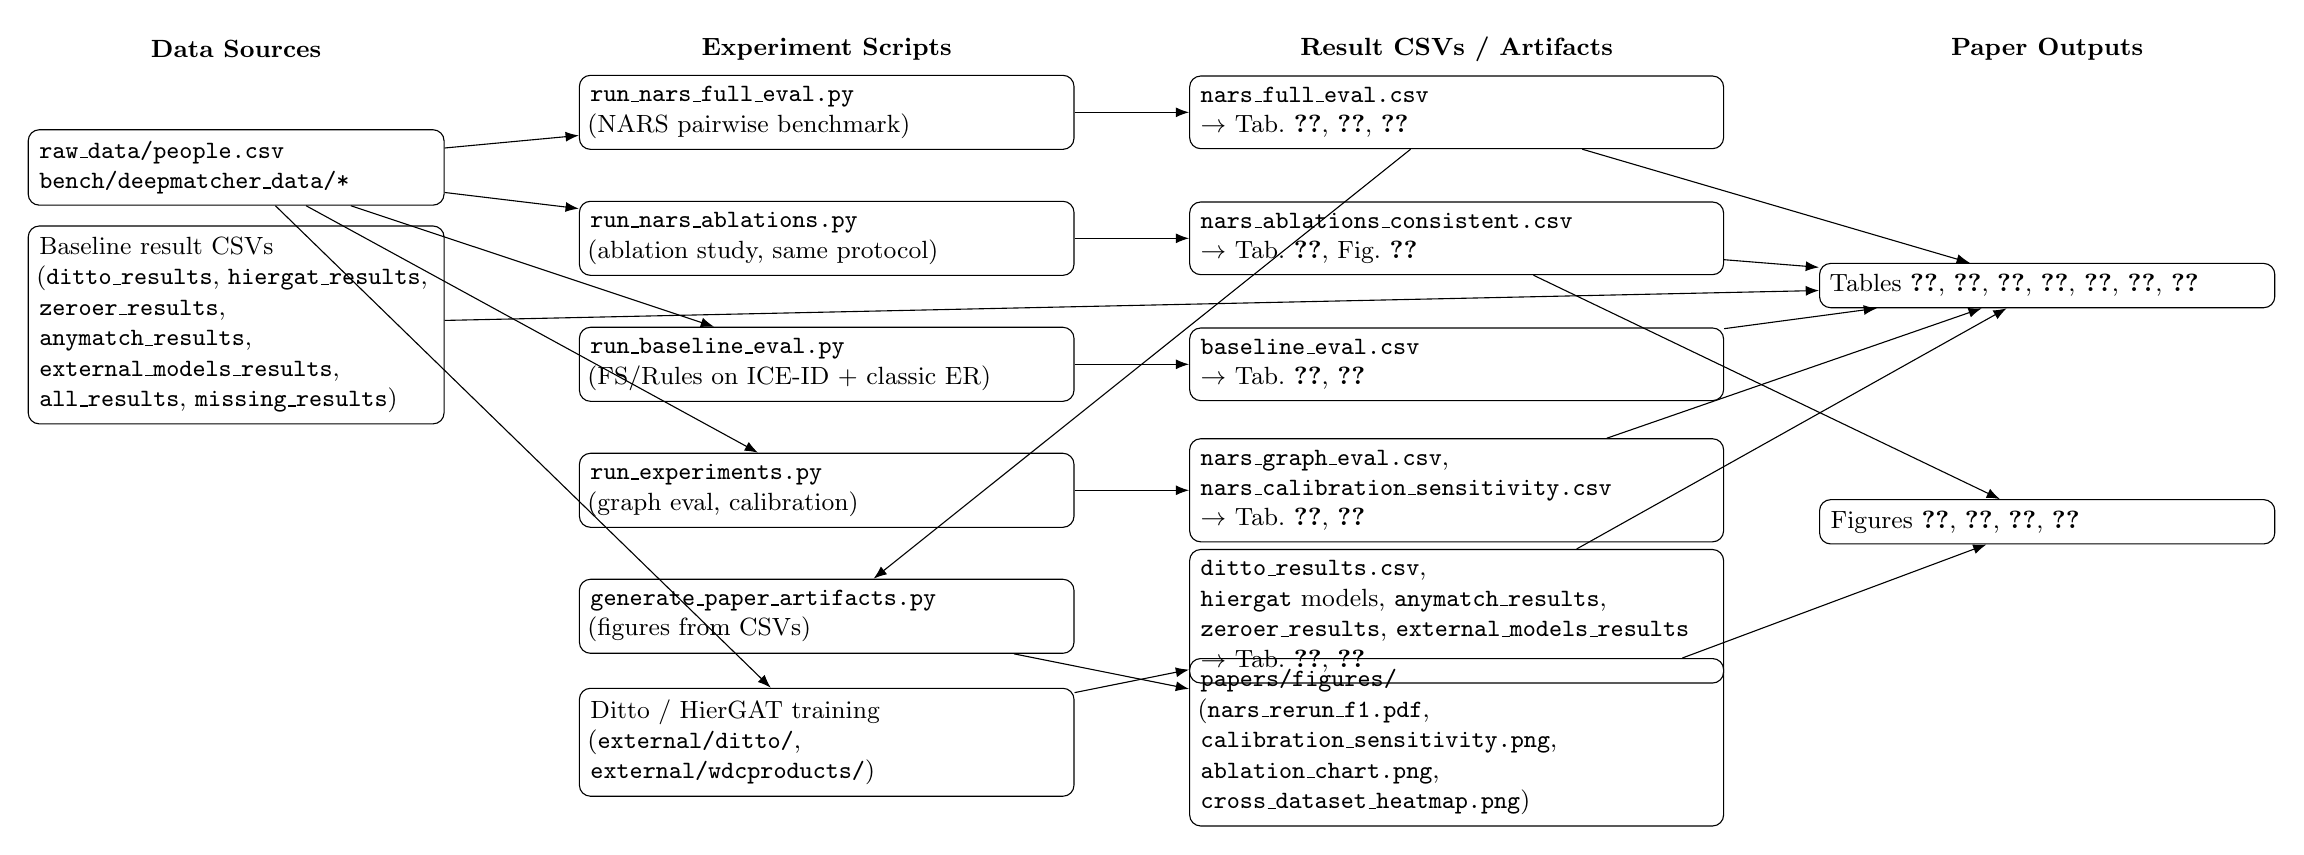
\begin{tikzpicture}[
    node distance=10mm and 12mm,
    >=Latex,
    box/.style={draw, rounded corners, align=left, font=\small, inner sep=4pt, text width=5.5cm},
    title/.style={font=\bfseries\small}
  ]
    \node[title] (c1) at (0, 4.0) {Data Sources};
    \node[title] (c2) at (7.5, 4.0) {Experiment Scripts};
    \node[title] (c3) at (15.5, 4.0) {Result CSVs / Artifacts};
    \node[title] (c4) at (23.0, 4.0) {Paper Outputs};

    % Column 1: Data Sources
    \node[box, text width=5cm] (d1) at (0, 2.5) {\texttt{raw\_data/people.csv}\\\texttt{bench/deepmatcher\_data/*}};
    \node[box, text width=5cm] (d2) at (0, 0.5) {Baseline result CSVs\\(\texttt{ditto\_results}, \texttt{hiergat\_results},\\\texttt{zeroer\_results}, \texttt{anymatch\_results},\\\texttt{external\_models\_results},\\\texttt{all\_results}, \texttt{missing\_results})};

    % Column 2: Scripts
    \node[box, text width=6cm] (s1) at (7.5, 3.2) {\texttt{run\_nars\_full\_eval.py}\\(NARS pairwise benchmark)};
    \node[box, text width=6cm] (s2) at (7.5, 1.6) {\texttt{run\_nars\_ablations.py}\\(ablation study, same protocol)};
    \node[box, text width=6cm] (s3) at (7.5, 0.0) {\texttt{run\_baseline\_eval.py}\\(FS/Rules on ICE-ID + classic ER)};
    \node[box, text width=6cm] (s4) at (7.5, -1.6) {\texttt{run\_experiments.py}\\(graph eval, calibration)};
    \node[box, text width=6cm] (s5) at (7.5, -3.2) {\texttt{generate\_paper\_artifacts.py}\\(figures from CSVs)};
    \node[box, text width=6cm] (s6) at (7.5, -4.8) {Ditto / HierGAT training\\(\texttt{external/ditto/}, \texttt{external/wdcproducts/})};

    % Column 3: Artifacts
    \node[box, text width=6.5cm] (a1) at (15.5, 3.2) {\texttt{nars\_full\_eval.csv}\\$\rightarrow$ Tab.~\ref{tab:nars_horizontal}, \ref{tab:comprehensive_baselines}, \ref{tab:iceid_results}};
    \node[box, text width=6.5cm] (a2) at (15.5, 1.6) {\texttt{nars\_ablations\_consistent.csv}\\$\rightarrow$ Tab.~\ref{tab:ablations}, Fig.~\ref{fig:ablation}};
    \node[box, text width=6.5cm] (a3) at (15.5, 0.0) {\texttt{baseline\_eval.csv}\\$\rightarrow$ Tab.~\ref{tab:iceid_results}, \ref{tab:comprehensive_baselines}};
    \node[box, text width=6.5cm] (a4) at (15.5, -1.6) {\texttt{nars\_graph\_eval.csv},\\\texttt{nars\_calibration\_sensitivity.csv}\\$\rightarrow$ Tab.~\ref{tab:nars_graph_eval}, \ref{tab:calibration_sensitivity}};
    \node[box, text width=6.5cm] (a5) at (15.5, -3.2) {\texttt{ditto\_results.csv},\\\texttt{hiergat} models, \texttt{anymatch\_results},\\\texttt{zeroer\_results}, \texttt{external\_models\_results}\\$\rightarrow$ Tab.~\ref{tab:comprehensive_baselines}, \ref{tab:iceid_results}};
    \node[box, text width=6.5cm] (a6) at (15.5, -4.8) {\texttt{papers/figures/}\\(\texttt{nars\_rerun\_f1.pdf},\\\texttt{calibration\_sensitivity.png},\\\texttt{ablation\_chart.png}, \texttt{cross\_dataset\_heatmap.png})};

    % Column 4: Outputs
    \node[box, text width=5.5cm] (p1) at (23.0, 1.0) {Tables~\ref{tab:iceid_results}, \ref{tab:comprehensive_baselines}, \ref{tab:nars_horizontal}, \ref{tab:sota_horizontal}, \ref{tab:ablations}, \ref{tab:nars_graph_eval}, \ref{tab:calibration_sensitivity}};
    \node[box, text width=5.5cm] (p2) at (23.0, -2.0) {Figures~\ref{fig:nars_rerun_f1}, \ref{fig:ablation}, \ref{fig:calibration}, \ref{fig:heatmap}};

    % Connections
    \draw[->] (d1) -- (s1);
    \draw[->] (d1) -- (s2);
    \draw[->] (d1) -- (s3);
    \draw[->] (d1) -- (s4);
    \draw[->] (d1) -- (s6);
    \draw[->] (s1) -- (a1);
    \draw[->] (s2) -- (a2);
    \draw[->] (s3) -- (a3);
    \draw[->] (s4) -- (a4);
    \draw[->] (s5) -- (a6);
    \draw[->] (s6) -- (a5);
    \draw[->] (a1) -- (s5);
    \draw[->] (a1) -- (p1);
    \draw[->] (a2) -- (p1);
    \draw[->] (a2) -- (p2);
    \draw[->] (a3) -- (p1);
    \draw[->] (a4) -- (p1);
    \draw[->] (a5) -- (p1);
    \draw[->] (a6) -- (p2);
    \draw[->] (d2) -- (p1);
  \end{tikzpicture}%
  }
  \caption{Provenance graph mapping data sources, scripts, result artifacts, and paper tables/figures. NARS, Fellegi--Sunter, and Rules results are produced by dedicated evaluation scripts; Ditto and HierGAT ICE-ID results come from direct training; other baseline results are from pre-computed CSVs.}
  \label{fig:nars_provenance_graph}
\end{figure}

\subsection{Metrics}
\begin{table}[H]
  \centering
  \small
  \begin{tabular}{lp{0.75\linewidth}}
    \toprule
    \textbf{Metric} & \textbf{Definition} \\
    \midrule
    Precision (P)  
      & $\displaystyle \frac{\mathrm{TP}}{\mathrm{TP} + \mathrm{FP}}$  
      — fraction of predicted matches that are correct. \\[0.3em]
    Recall (R)     
      & $\displaystyle \frac{\mathrm{TP}}{\mathrm{TP} + \mathrm{FN}}$  
      — fraction of true matches that are found. \\[0.3em]
    F$_1$ Score    
      & $2 \cdot \frac{P \cdot R}{P + R}$  
      — harmonic mean of precision and recall. \\[0.3em]
    Accuracy (Acc) 
      & $\displaystyle \frac{\mathrm{TP} + \mathrm{TN}}{\mathrm{TP} + \mathrm{TN} + \mathrm{FP} + \mathrm{FN}}$  
      — proportion of correct predictions. \\[0.3em]
    Threshold (Thr)
      & Calibrated score cutoff $\tau$ separating matches vs.\ non-matches. \\[0.3em]
    AUC           
      & Area under the ROC curve — ranking quality over all thresholds. \\[0.3em]
    ARI-CC        
      & Adjusted Rand Index on connected-component clustering of thresholded graph. \\[0.3em]
    ARI-AG        
      & Adjusted Rand Index on agglomerative clustering of pairwise scores. \\[0.3em]
    Precision@k (P@k) 
      & Precision among the top-$k$ highest-scoring pairs, where $k$ equals the number of positives in slice. \\[0.3em]
    Recall@k (R@k)    
      & Recall among the top-$k$ highest-scoring pairs. \\
    \bottomrule
  \end{tabular}
  \caption{Definitions of the evaluation metrics used in Tables~\ref{tab:nars_horizontal} and~\ref{tab:sota_horizontal}.}
  \label{tab:metric_definitions}
\end{table}

\subsection{Benchmark-specific NARS preprocessing (classic ER datasets)}
ICE-ID preprocessing remains unchanged and follows the rules described earlier in the paper. For the classic two-table ER benchmarks, we replaced the generic token-overlap preprocessing with dataset-specific judgments so that NARS can use the fields that define matches in each dataset.

\textbf{Shared normalization and scoring.} Text fields are lowercased, stripped, and normalized by removing non-alphanumeric characters and collapsing whitespace. Similarity is the maximum of token Jaccard overlap and SequenceMatcher ratio. For each text field we emit:
\texttt{field\_exact} if normalized strings match, else
\texttt{field\_sim\_high} ($\ge$ 0.90),
\texttt{field\_sim\_med} ($\ge$ 0.75),
\texttt{field\_sim\_low} ($\ge$ 0.50), or
\texttt{field\_sim\_vlow} (otherwise).
Numeric fields are parsed by extracting the first numeric token. We emit \texttt{field\_exact} if absolute difference $\le$ 0.01, \texttt{field\_close} if absolute difference $\le$ a dataset-specific threshold or relative difference $\le$ 0.05, and \texttt{field\_far} if relative difference $\ge$ 0.20. Year fields are parsed from 4-digit years and emit \texttt{field\_same} (diff=0), \texttt{field\_close} (diff $\le$ 1), or \texttt{field\_far}. Time fields accept seconds or \texttt{mm:ss} and emit \texttt{time\_same} (diff=0), \texttt{time\_close} (diff $\le$ 5s), or \texttt{time\_far}. Phone fields compare digits only and emit \texttt{phone\_exact}, \texttt{phone\_last7}, or \texttt{phone\_mismatch}. Address numbers emit \texttt{addr\_num\_match} or \texttt{addr\_num\_diff} when parseable.

\textbf{Dataset-specific judgments.}
\begin{itemize}
  \item \textbf{Abt--Buy:} \texttt{name}, \texttt{description} (text), \texttt{price} (numeric; abs $\le$ 1.0 or rel $\le$ 0.05).
  \item \textbf{Amazon--Google:} \texttt{title}, \texttt{manufacturer} (text), \texttt{price} (numeric; abs $\le$ 1.0 or rel $\le$ 0.05).
  \item \textbf{DBLP--ACM / DBLP--Scholar:} \texttt{title}, \texttt{authors}, \texttt{venue} (text), \texttt{year} (same/close/far).
  \item \textbf{iTunes--Amazon:} \texttt{Song\_Name}, \texttt{Artist\_Name}, \texttt{Album\_Name}, \texttt{Genre} (text), \texttt{Price} (numeric; abs $\le$ 0.5 or rel $\le$ 0.05), \texttt{Time} (time), \texttt{Released} and \texttt{CopyRight} (year).
  \item \textbf{Walmart--Amazon:} \texttt{title}, \texttt{category}, \texttt{brand}, \texttt{modelno} (text), \texttt{price} (numeric; abs $\le$ 1.0 or rel $\le$ 0.05).
  \item \textbf{Beer:} \texttt{Beer\_Name}, \texttt{Brew\_Factory\_Name}, \texttt{Style} (text), \texttt{ABV} (numeric; abs $\le$ 0.3 or rel $\le$ 0.05).
  \item \textbf{Fodors--Zagats:} \texttt{name}, \texttt{addr}, \texttt{city}, \texttt{type}, \texttt{class} (text), plus phone and address-number judgments.
\end{itemize}

\textbf{Data alignment for DeepMatcher splits.} For these benchmarks, pair IDs correspond to the source tables (e.g., \texttt{abt.csv}/\texttt{buy.csv}, \texttt{amazon.csv}/\texttt{google.csv}), so we align record IDs to the pair indices before applying the standard right-table offset to make IDs globally unique. This ensures that all training and evaluation pairs map to actual records.

\textbf{Thresholding.} ICE-ID uses the original median-based separation of positive/negative validation scores. For classic ER benchmarks, we select a per-dataset threshold that maximizes validation F$_1$ to accommodate extreme class imbalance.

\subsection{NARS Background}
\label{subsec:nars_background}
NARS uses \emph{channels} to transform external information into Narsese (its internal knowledge representation). A channel can process information of any modality---strings for natural language, matrices for visual signals---under a single principle: compounding atomic inputs (e.g., words in a sentence or pixels in an image) into structured terms. For the problem discussed here, channels process census records.

Compounding is guided by NARS's memory-based attention allocation rather than brute-force enumeration. However, when only census data are provided, NARS lacks the semantics of domain concepts (e.g., farm locations), so additional preprocessing of raw records is required. Future work could supply spatial and temporal relationships directly, allowing NARS to ground input semantics through geographical and historical context.

In summary, our approach adapts the compound generation method from NARS channels and the truth-value calculus to entity resolution, while omitting memory management and goal-driven inference components. This focused adaptation enables direct comparison with standard ML baselines on ER benchmarks.

\subsubsection{Channel}

The NARS channel maintains a short-term cache of recent inputs, each consisting of multiple atomic sensations. From this cache the channel constructs two types of compounds: \emph{spatial compounds}, which group co-occurring sensations into a single moment, and \emph{temporal compounds}, which capture implication relationships between spatial compounds for prediction. Because census records lack short-term sequential structure, we use only spatial compounds.
Rather than enumerating all combinations of atomic sensations, the channel forms a compound as a whole and then determines which parts can be eliminated.

\subsubsection{Truth-Value}

In NARS, the truth-value of a judgment quantifies both positive and negative evidence. Given $w_+$ units of positive evidence and $w_-$ units of negative evidence, the truth-value $(f, c)$ is defined as $f=w_+/(w_++w_-)$ and $c=(w_++w_-)/(w_++w_-+k)$, where $f \in [0,1]$ (the \emph{frequency}) is the proportion of positive evidence and $c \in [0,1]$ (the \emph{confidence}) measures how much existing evidence there is relative to $k$ hypothetical future observations. Higher $f$ indicates stronger positive support; higher $c$ indicates that $f$ is less likely to change with new evidence.

\subsubsection{The Expectation of Truth-Values}

Because the truth-value is two-dimensional, NARS defines a scalar summary called \emph{expectation}: $e = c(f-0.5) + 0.5$, with $e\in [0,1]$. Values of $e$ near 1 indicate a judgment that is both true and reliable; values near 0 indicate a judgment that is both false and reliable. When $e \approx 0.5$, the system is either ignorant ($f \approx 0.5$) or lacks sufficient evidence ($c$ is low).

\subsubsection{The Revision of Truth-Values}

When two independent sources provide truth-values for the same judgment, NARS integrates them via \emph{revision}: $w_+=w_+^{(1)}+w_+^{(2)}$, $w_-=w_-^{(1)}+w_-^{(2)}$, with $f$ and $c$ recomputed from the pooled evidence counts.

\subsubsection{Pilot Hyperparameter Tuning}

\emph{Note: this subsection describes an early pilot procedure used to select NARS hyperparameters before the final benchmark protocol (Section~\ref{sec:methods}) was fixed.}

Census records up to 1899 served as training data and records after 1899 as test data. Records were sorted by individual so that records from the same person appeared consecutively. For each record, $m$ subsequent rows were paired with it, yielding both positive pairs (same person) and negative pairs (different persons).

At test time, $x$ individuals were sampled from the test set and all pairwise match scores among their records were computed. A symmetric threshold $\delta$ around 0.5 was swept: pairs with score $> 0.5 + \delta$ were predicted as matches and pairs with score $< 0.5 - \delta$ as non-matches, and F$_1$ was computed for each $\delta$. Default settings: $1/10{,}000$ of training data, $x=1{,}000$ test individuals, $m=5$ neighbor rows, and 10 reference patterns.

Increasing the number of reference patterns improved reliability, while varying the training proportion and observation scope had less consistent effects.

\textbf{Handcrafted Rules (pilot-era rule set).} The following field-level judgments were used in early pilot experiments. The final benchmark uses the extended judgment vocabulary described in Section~\ref{sec:methods} (which adds graded birthyear thresholds, geographic hierarchy levels, and temporal gap judgments). When processing a record pair, the pilot rules generate:

\textit{\textbf{Heimild}}: Emits \texttt{differ\_in\_X\_years}, where $X$ is the absolute difference in census year between the two records.

\textit{\textbf{nafn\_norm}}: Emits \texttt{same\_nafn\_norm} or \texttt{different\_nafn\_norm} based on whether the normalized full names match. The same logic applies to \textbf{\textit{first\_name}}, \textbf{\textit{patronym}}, and \textbf{\textit{surname}}.

\textit{\textbf{Birthyear}}: Emits \texttt{same\_birthyear} or \texttt{different\_birthyear} based on whether the birth years match.

\textit{\textbf{Sex}}: Emits \texttt{same\_sex} or \texttt{different\_sex} based on whether the sex values match.

\textit{\textbf{Status}}: Because social status is categorical rather than binary, two judgments are emitted: \texttt{status\_is\_X} and \texttt{status\_is\_Y}, where $X$ and $Y$ are the status values from each record (unordered).

\textit{\textbf{Marriagestatus}}: Emits \texttt{same\_marriagestatus} or \texttt{different\_marriagestatus} based on whether the marital status values match.

\textit{\textbf{Farm}}: Emits \texttt{same\_farm} or \texttt{different\_farm} based on whether the farm IDs match. The same logic applies to \textit{\textbf{county}}, \textit{\textbf{parish}}, and \textit{\textbf{district}}.

\textit{\textbf{Label}}: The ground-truth indicator: records are from the same individual if and only if they share the same \texttt{person} ID.

\end{document}
